\section{Theoretical Analysis}
\label{sec:analysis}

In this section we will analyse theoretical our bandpass filter using OP AMP. \\
To do so, and because there were several things to be analysed, we divided the theoretical analysis in the following subsections that explain the different sectors that our circuit has and also each one will be detailed separately.\\

\subsection{Transfer function computation}

%BANDPASS FREQUENCY
\begin{table}[H] \centering
\begin{tabular}{|
>{\columncolor[HTML]{FFCC67}}l |c|}
\hline
\multicolumn{2}{|l|}{\cellcolor[HTML]{EABD8B}Name - Value} \\ \hline
LowFreq BandPass & 4.545455e+03 \\ \hline
HighFreq BandPass & 9.090909e+03 \\ \hline
Central Freq & 6.428243e+03 \\ \hline

\end{tabular}
\caption{BANDPASS FREQUENCY}
\end{table}

%WO FREQUENCY GAIN
\begin{table}[H] \centering
\begin{tabular}{|
>{\columncolor[HTML]{FFCC67}}l |c|}
\hline
\multicolumn{2}{|l|}{\cellcolor[HTML]{EABD8B}Name - Value} \\ \hline
Central Freq (Hz) & 1.023087e+03 \\ \hline
Gain Central Freq (dB) & 3.656460e+01 \\ \hline

\end{tabular}
\caption{WO FREQUENCY GAIN}
\end{table}

%FIGURE GAIN
\begin{figure}[H] 
\centering
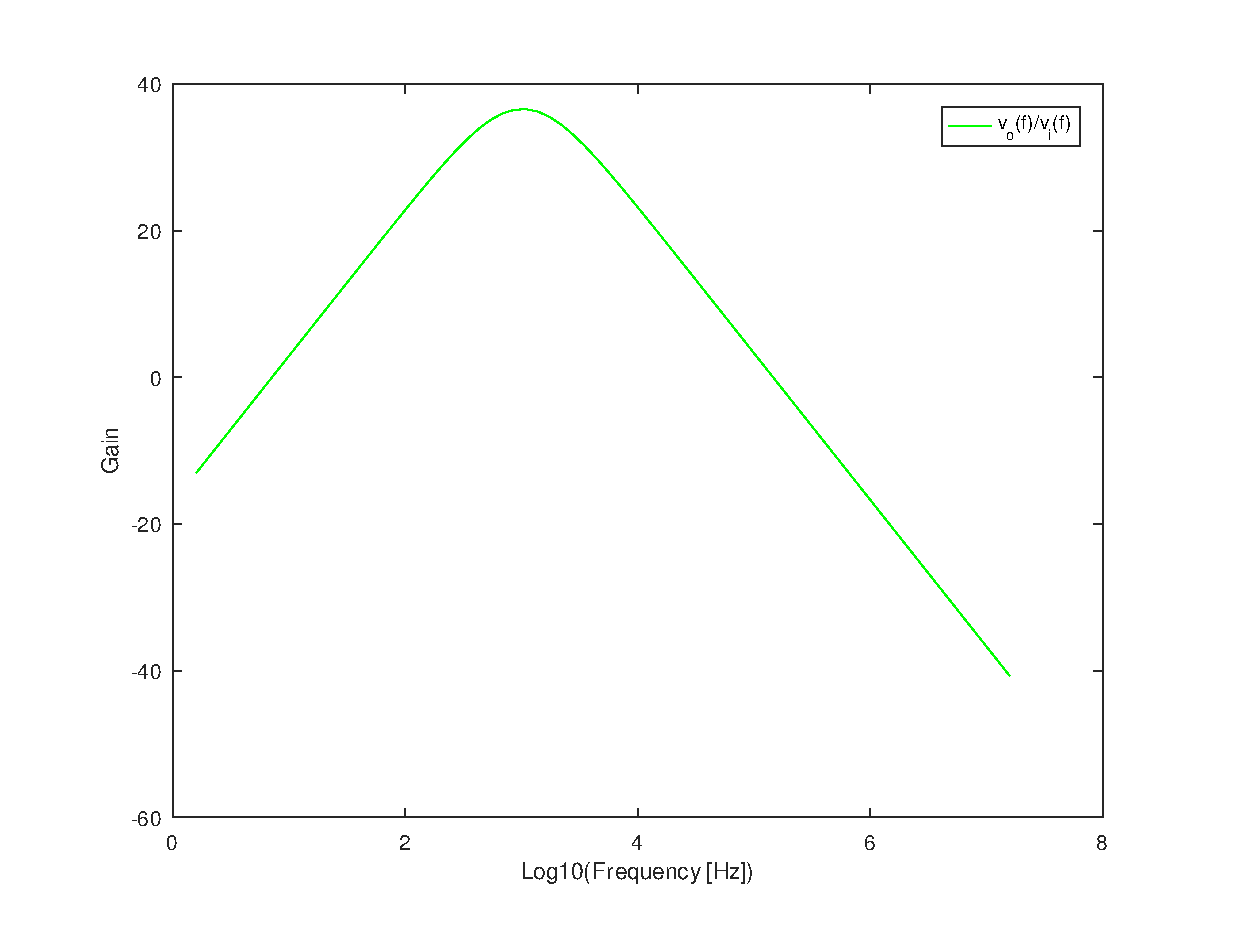
\includegraphics[width = 8cm]{gain.eps} 
\caption{Gain}
\label{gain}
\end{figure}

%FIGURE PHASE
\begin{figure}[H] 
\centering
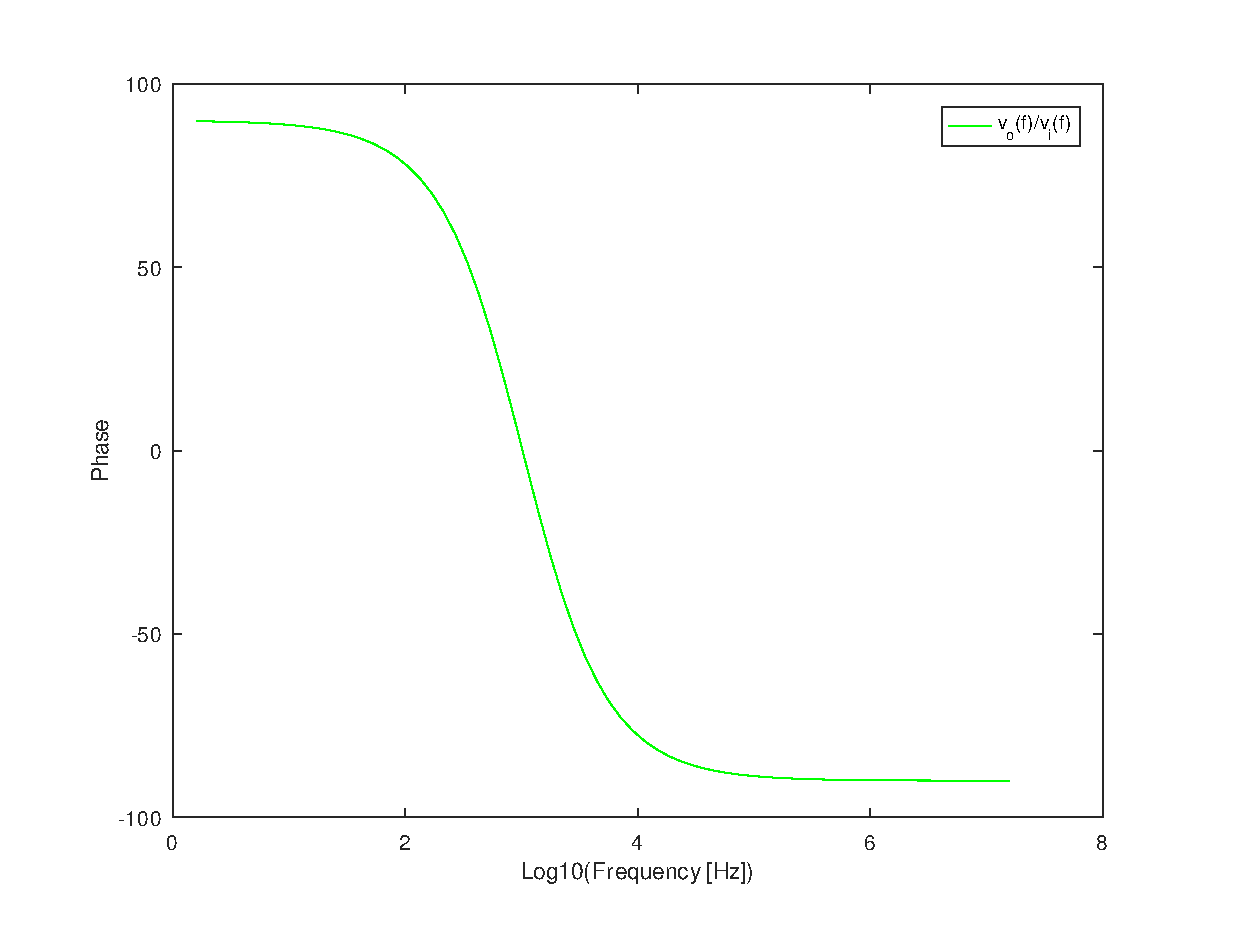
\includegraphics[width = 8cm]{phase.eps} 
\caption{Phase}
\label{phase}
\end{figure}

\subsection{Input and Output Impedances}

%IMPEDANCES
\begin{table}[H] \centering
\begin{tabular}{|
>{\columncolor[HTML]{FFCC67}}l |c|}
\hline
\multicolumn{2}{|l|}{\cellcolor[HTML]{EABD8B}Name - Value} \\ \hline
Z in & 1.000000e+03 + -7.071068e+02j \\ \hline
Z out & 6.666667e+02 + -4.714045e+02j\\ \hline

\end{tabular}
\caption{IMPEDANCES}
\end{table}


%LEO
In this section, a theoretical analysis of the circuit shown in section 1 was conducted. The OP Amp was considered ideal (internal impedance between v+ and v- is infinite, which means no current flows through it and vos=0 or in other words v+ = v-). So, in order to build a bass pand filter, a capactior was connected in series (C1) with the input voltage which will function as a high pass filter (for low frequencies, the impedance goes to infinity and the capacitor is basically an open circuit)  and other capacitor (C2) was connected in parallel with the output voltage, functioning as a low pass filter (for high impedances, the impedance goes to 0 and the capacitor is basically a short circuit). To sum up, this circuit consists of a high pass filter, a signal amplifier and a low pass filter in series.

